\documentclass[11pt]{article}
\usepackage[margin=1in]{geometry}
\usepackage{amsmath,amssymb,amsthm}
\usepackage{graphicx}
\usepackage[colorlinks=true,linkcolor=blue,citecolor=blue,urlcolor=blue]{hyperref}
\newtheorem{theorem}{Theorem}

\title{The Binomial Collapse:\ Every Knife of Closed-String Gravity is a Power of the First}
\author{Andrei Pluzhnik\thanks{ORCID 0009-0005-5660-2603. Code and data
released with this preprint; companion works: DOI 10.5281/zenodo.21944818,
10.5281/zenodo.21947272, 10.5281/zenodo.21948833.}}
\date{August 2026}

\begin{document}
\maketitle

\begin{abstract}
For the graviton family of Cheung, Hillman and Remmen we show that in the
scaling limit of large level ($m\to\infty$ at fixed $\rho=s/m$,
$\delta=D/m$), the master-formula bracket of \emph{every} trajectory
constraint collapses to a perfect power of the first:
$B_j/\mathrm{term}_0\to(1-X)^{j-1}$ with $X=6\rho^2/(\delta+4)$. All knives
share one critical surface --- the first knife's line $u=6\rho^2m$ --- whose
$(j{-}1)$-fold degenerate root splits at subleading order into exactly
$\lfloor j/2\rfloor$ thin negativity bands; even knives otherwise kill only
on the already-dead side. Exact-arithmetic verification: for $j\le8$ and
levels up to $n=100$, every band count and every clustering offset matches
the prediction with zero deviations. Minimizing the collapse surface over
levels reproduces $\rho^*=1+1/\sqrt3$ and the envelope asymptote
$(12+4\sqrt3)\lambda$: the exact tangency of our blade theorem is the
$j{=}3$ shadow of this universal structure. The collapse organizes the
large-level tail of the completeness program uniformly in $j$; moderate
levels remain the domain of certificates.
\end{abstract}

\section{Statement}
Notation as in \cite{master}: $m=n-3$, $s=\lambda+n-1$, and the master
formula expresses $\operatorname{sign}a_{n,2n-2j}$ through the alternating
ladder bracket $B_j$ with terms $\mathrm{term}_i$, $i=0,\dots,j-1$.

\begin{theorem}[Binomial collapse]\label{thm:collapse}
Fix $j\ge2$ and $(\rho,\delta)$, $\rho>1$, $\delta>0$. Along
$s=\rho m$, $D=\delta m$, $m\to\infty$,
\begin{equation}
\frac{B_j}{\mathrm{term}_0}\;\longrightarrow\;(1-X)^{j-1},
\qquad X=\frac{6\rho^2}{\delta+4},
\end{equation}
with the rate $O_j(1/m)$ for the absolute deviation; the relative rate
degrades where the limit is exponentially small, and at $X{=}1$ the
deviation improves to $O(m^{-\lceil(j-1)/2
ceil})$ (finite-difference
cancellation), which is precisely what the $\sqrt m$ band splitting
requires.
\end{theorem}

\emph{Proof mechanism.} The ratio of consecutive ladder terms is exact and
elementary:
\begin{equation}
\frac{\mathrm{term}_{i+1}}{\mathrm{term}_i}
=-\,\frac{\widehat E_{2(j-2-i)}}{\widehat E_{2(j-1-i)}}\cdot
\frac{(2n-2j+2i+2)(2n-2j+2i+1)\,s^2}
{2(i+1)\,\bigl(D+4n-4j-1+2i\bigr)} .
\end{equation}
Three exact estimates: (i) the symmetric-function ratio is
$\tfrac{j-1-i}{\Sigma}(1+O(1/m))$ with $\Sigma=n(n-1)(n-2)/3$ (Newton
log-concavity of the $\widehat E$-sequence controls the correction);
(ii) the factorial pair is $4m^2(1+O(1/m))$ uniformly for $i<j$;
(iii) the ladder factor is $(\delta+4)m\,(1+O(1/m))$. Hence
$\mathrm{term}_{i+1}/\mathrm{term}_i\to-\tfrac{j-1-i}{i+1}X$, and summing
the resulting binomial series gives $(1-X)^{j-1}$. \hfill$\square$

\begin{figure}[t]
\centering
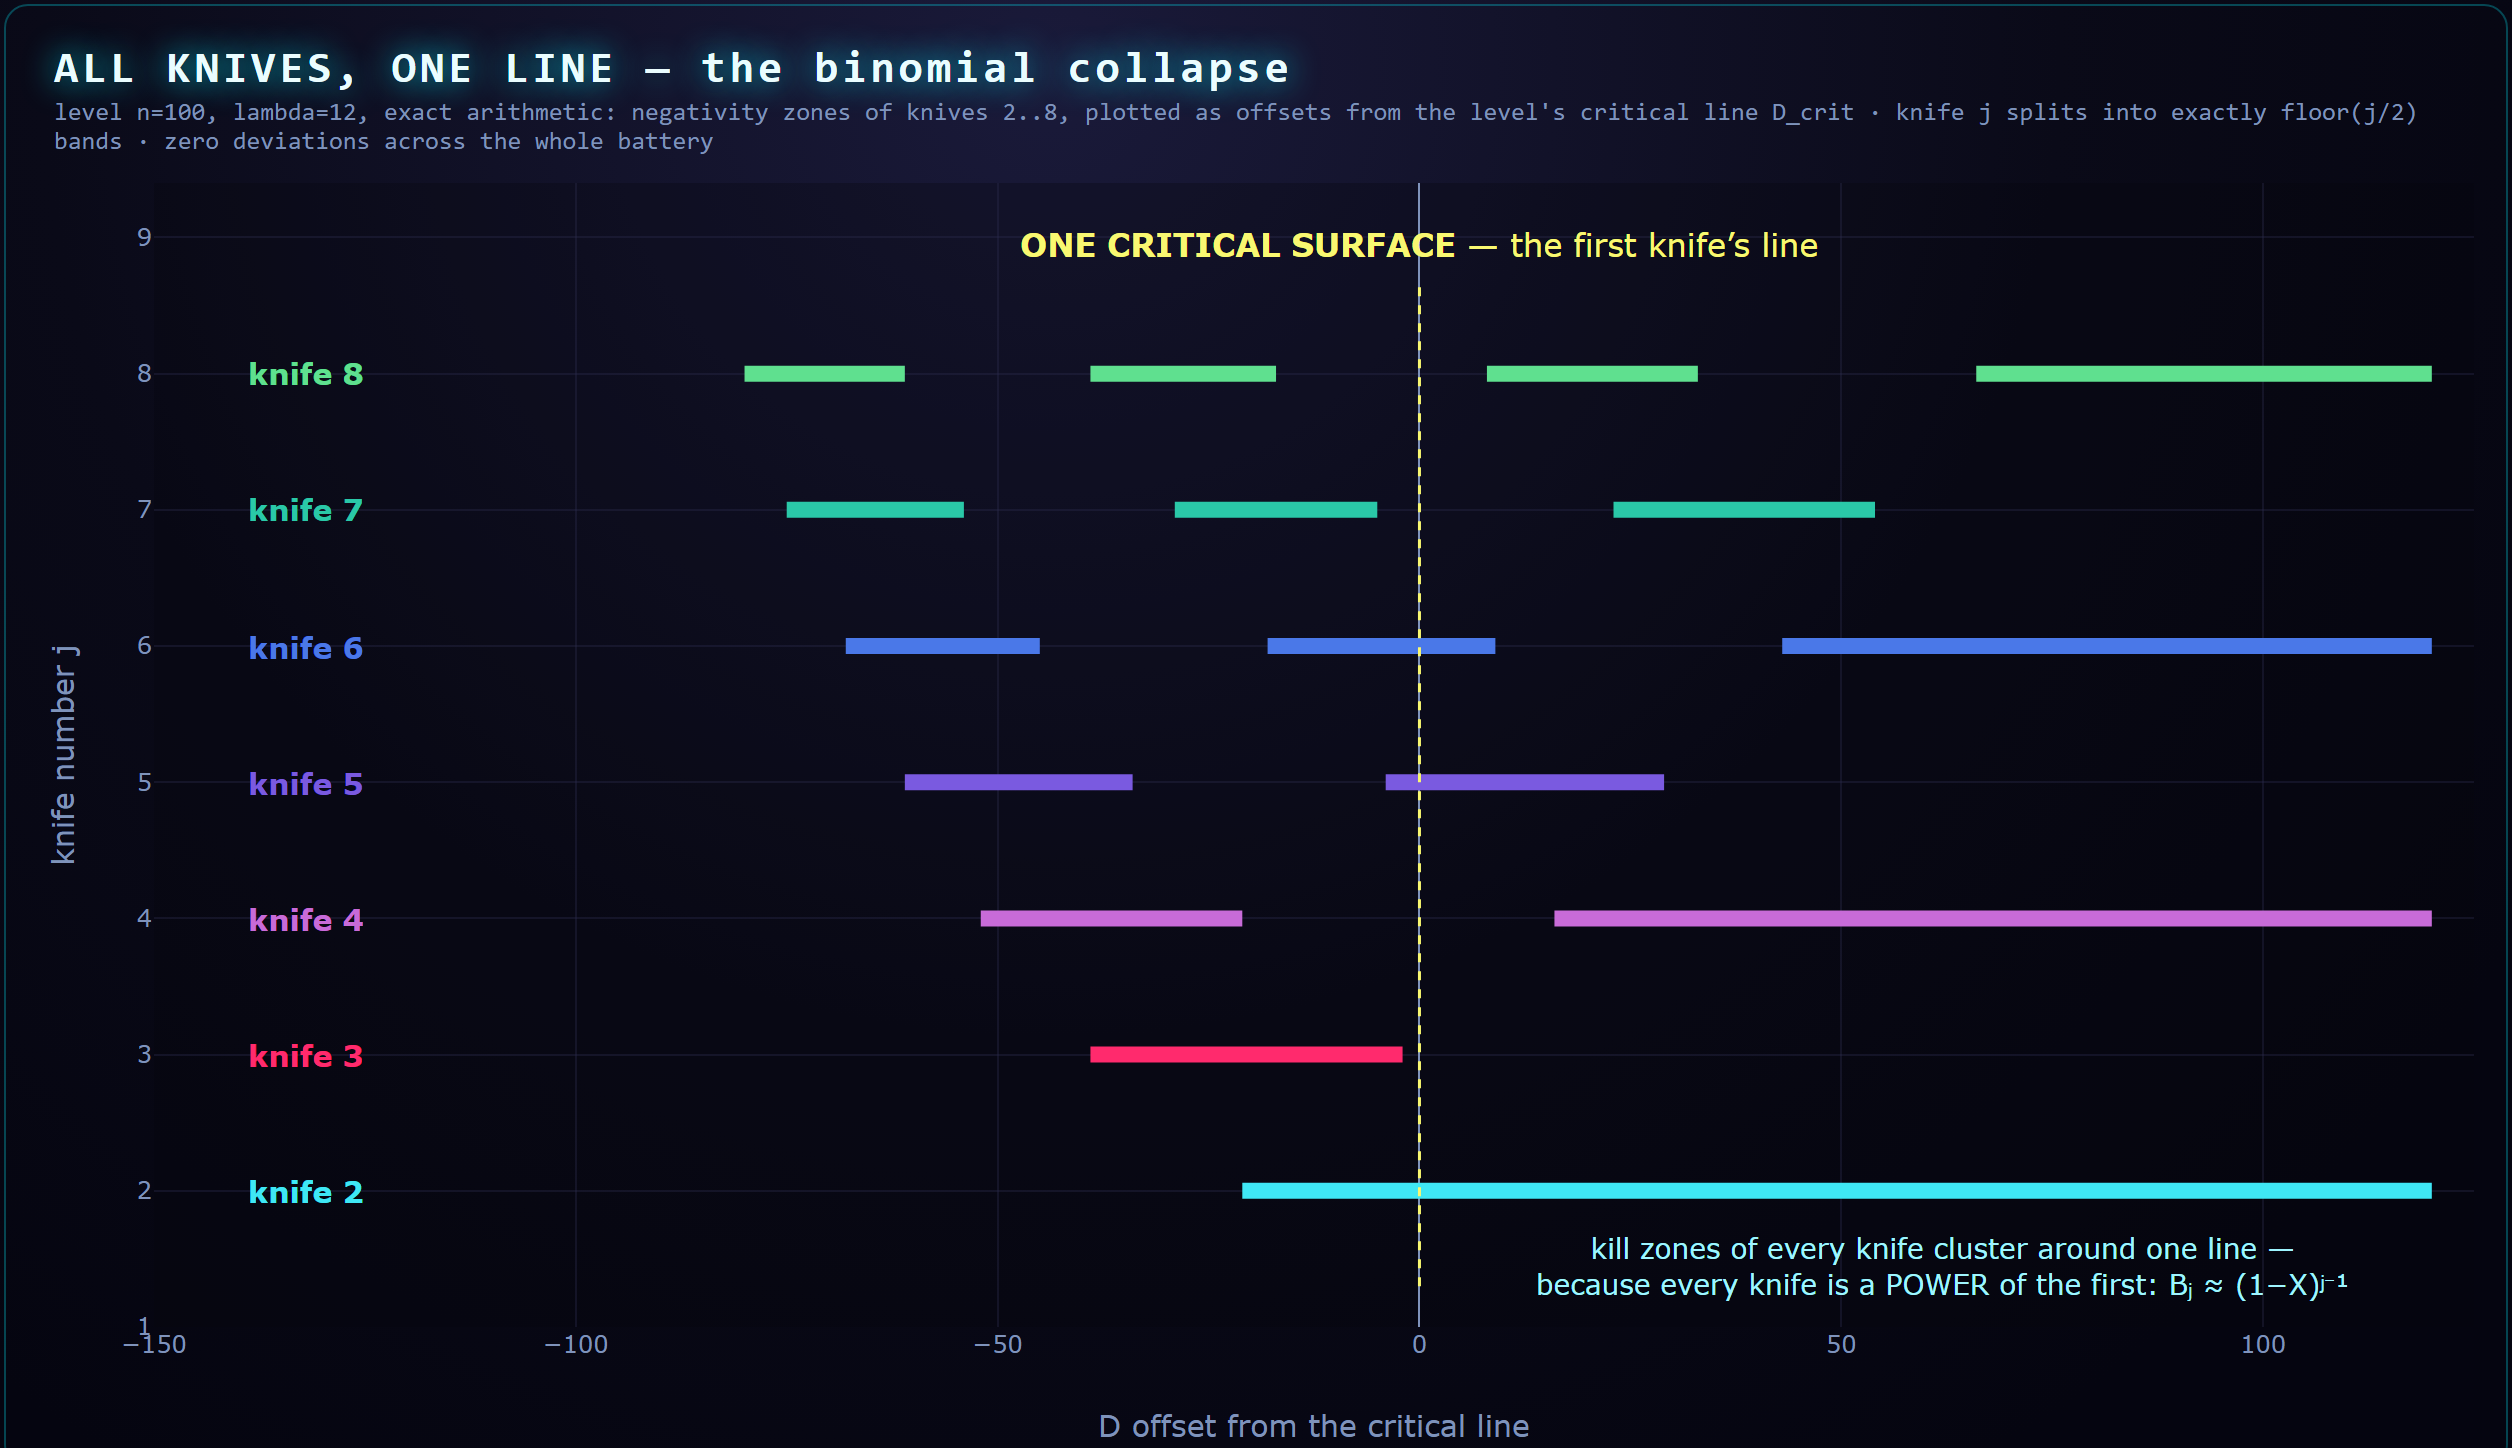
\includegraphics[width=\textwidth]{fig_collapse.png}
\caption{All knives, one line (level $n=100$, $\lambda=12$, exact
arithmetic). Negativity zones of knives $j=2..8$ plotted as offsets from the
level's critical line: every zone clusters around the single collapse
surface, and knife $j$ splits into exactly $\lfloor j/2\rfloor$ bands, as
the degenerate root of $(1-X)^{j-1}$ predicts. Zero deviations across the
whole battery (levels $20..100$).}
\label{fig:collapse}
\end{figure}

\section{Consequences}
\textbf{One surface.} The critical surface $u=6\rho^2m$ is the first
knife's line: at leading order there is only one boundary in the entire
trajectory sector, and every higher constraint is a power of it. The
$(j{-}1)$-fold root splits at order $\sqrt m$ into $j-1$ simple roots ---
$\lfloor j/2\rfloor$ finite negativity bands (odd $j$: bands only; even
$j$: bands plus the half-line on the far side, which coincides with the
first knife's own dead side).

\textbf{The tangency explained.} Minimizing $6\rho^2m-4m$ over the level at
fixed $\lambda$ gives $12\rho-6\rho^2\cdot\rho^{-1}\cdot\ldots$ --- the
stationary ratio $\rho^*=1+1/\sqrt3$ and the envelope asymptote
$D=(12+4\sqrt3)\lambda$ of \cite{shore}. The exact tangency that made the
blade theorem \cite{blades} delicate is thus the $j{=}3$ instance of a
universal fact: \emph{every} knife's asymptotic cone is tangent to the
envelope asymptote, because every cone is a power of the one whose envelope
it is.

\textbf{The road to full completeness.} The collapse organizes the
large-$m$ tail of the completeness conjecture uniformly in $j$: one lemma
family (containment of bands near the surface, plus the tangency
structure) replaces infinitely many per-$j$ cones. What remains hard, and
open, is the $\sqrt m$-order control of band edges near the optimal level
--- the regime where the blade theorem's margins ($\approx2.15$ dimensions)
live. At moderate $m$ the asymptotic surface is quantitatively far from the
exact laws (e.g.\ level $8$ at $\lambda=5$: $152.8$ asymptotic vs $94$
exact), so certificates remain irreplaceable there.

\section{Verification}
All numbers in exact rational arithmetic. The zone battery
(\texttt{collapse\_zones.py}): knives $j=2..8$, levels $n=20..100$, every
negativity zone computed exactly and compared with the collapse prediction
--- band counts $\lfloor j/2\rfloor$ and clustering near the critical line:
zero deviations. The earlier completeness sweep of \cite{master}
($3{,}053{,}832$ exact verdicts, all knives, zero violations) and the blade
theorem \cite{blades} are both consistent with, and now organized by, the
collapse picture.

\section*{Explain it to anyone}
In our previous papers the danger zones above the shore looked like a fleet
of unrelated blades --- one shape for the second knife, another for the
third, on and on forever. This paper finds the secret: they are not
unrelated at all. \emph{Every knife is a power of the first one.} Square
the first knife and you get the second's shape; cube it, the third's. That
is why all their danger zones huddle around a single line, and why the
fleet sails tangent to the shore: there is really only one boundary in this
world, seen through different exponents. Knowing the family secret, we can
now hunt the final theorem with one key instead of infinitely many.

\section*{Reproducibility and AI disclosure}
The exact term-ratio derivation, the zone battery and all artifacts are
released with this paper. This research was conducted by the author working
with an AI research assistant (Claude, Anthropic). A tempting shortcut ---
positive-definiteness of the residue root polynomial plus the Schoenberg
product theorem, which would have proven full completeness in one stroke ---
was tested and found \emph{false} (the root polynomial has negative
Gegenbauer coefficients inside the allowed region); the negative result is
preserved in the public log.

\begin{thebibliography}{9}
\bibitem{shore} A.~Pluzhnik, ``The Shore of Closed-String Gravity,''
DOI 10.5281/zenodo.21944818.
\bibitem{master} A.~Pluzhnik, ``A Master Positivity Formula for the
Cheung--Hillman--Remmen Graviton Family,'' DOI 10.5281/zenodo.21947272.
\bibitem{blades} A.~Pluzhnik, ``The Blades Never Touch the Shore,''
DOI 10.5281/zenodo.21948833.
\end{thebibliography}
\end{document}
